\documentclass[11pt]{article}

\usepackage[margin = 1.0in]{geometry}
\usepackage[spanish]{babel}
\usepackage{here}
\usepackage{amsmath}
\usepackage{amssymb}
\usepackage{mathtools}
\usepackage{bm}
\usepackage{enumitem}
\usepackage{sectsty}
\usepackage{graphicx}
\usepackage[colorlinks=true,urlcolor=blue]{hyperref}
\usepackage{authblk}
\usepackage{caption}
\usepackage{fancyvrb}
\usepackage{relsize}
\usepackage{minted}
\usepackage{verbatim}
\usepackage{subcaption}

\title{Inteligencia Artificial Generativa - Obligatorio 1}
\author{Matias Molinolo \and Martina Diaz}

\date{\today}

\begin{document}
\maketitle
\thispagestyle{empty}
\newpage
\tableofcontents
\newpage

\section{Estimación de distribuciones}

\subsection{Dataset 1: Tennis}
marti vos escribis este 
ok gracias $<$3
:)
\subsection{Dataset 2: Iris}
y este

\section{Modelos generativos}
\subsection{NADE: Neural Autoregressive Distribution Estimator}

Intentamos reproducir en Pytorch la arquitectura del NADE propuesta por \cite{nade}, con ciertas modificaciones que resultaron de la prueba y error de la arquitectura.

Uria et al. propone una arquitectura autorregresiva que parte de la base que cualquier distribución $D$-dimensional $p$ puede expresarse como un producto de distribuciones unidimensionales \cite{nade}:

$$
p(\boldsymbol{x}) = \prod_{d=1}^{D}p(x_{o_d} \mid \boldsymbol{x}_{o_{<d}})
$$

Nuestra arquitectura usa 192 unidades ocultas, en vez de las 500 propuestas en el paper original. Esto se debe a que tras varios ensayos, encontramos que este número daba una buena performance y un tiempo de ejecución significativamente menor al de la arquitectura original del paper. 

El NADE fue entrenado con datos binarizados del dataset MNIST, donde se filtraron todos aquellos elementos que no pertenecían a la clase que quería generarse.

Luego de entrenarlo por 50 epochs, hicimos un muestreo de la distribución estimada por el NADE, obteniendo el siguiente resultado:

\begin{figure}[h]
    \centering
    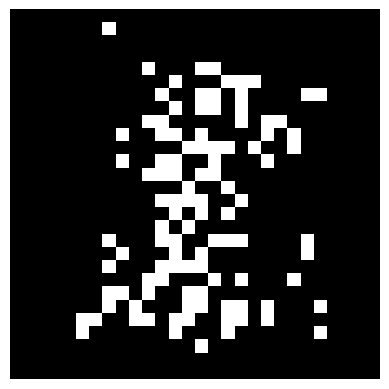
\includegraphics[width=0.3\textwidth]{NADE/nade_generation.png}
    \caption{Distribución estimada por el NADE}
    \label{fig:nade_gen}
\end{figure}

Podemos ver que no es una representación acertada, pero podría decirse que se asemeja a la clase original de los 1. Esto puede deberse a falta de entrenamiento u otros factores.
\newpage
\subsection{VAE: Variational Autoencoder}

A partir del tutorial de Doersch \cite{vae}, entrenamos un VAE y un VAE condicional, es decir, que genera una nueva imagen dada una clase específica.

Nuevamente, entrenamos esta red con el dataset del MNIST, pero esta vez sin filtrar ni binarizar.

Es interesante visualizar el espacio latente del VAE y el VAE condicional, que podemos observar en las siguientes figuras:

\begin{figure}
\begin{subfigure}[h]{0.45\linewidth}
    \centering
    \includegraphics{}
    \caption{Caption}
    \label{fig:enter-label}
\end{subfigure}
\begin{subfigure}[h]{0.45\linewidth}
    \centering
    \includegraphics{}
    \caption{Caption}
    \label{fig:enter-label}
\end{subfigure}
\end{figure}

\newpage
\section{Obligatorio 2}

\newpage

\bibliographystyle{ieeetr}
\bibliography{refs}

\end{document}
